\subsection{Disturbance attenuation}

In this subsection, we need to design a controller which both tracks the reference signal and attenuates the disturbances.

The transfer function of the system is:

$$G(s) = \frac{20}{(s+1)((\frac{s}{20})^2+\frac{s}{20}+1)}$$

The disturbance transfer function is:

$$G_d(s) = \frac{10}{s+1}$$

The purpose of this subsection is to designed the prefilter function and the feedback function ($F_r$ and $F_y$) with the following specifications:

\begin{shortitemize}
    \item Rise time $t_r \leq 0.2$ s
    \item Overshoot $D(\%) \leq 10\%$
    \item Step in the disturbance:
        $$|y(t)| \leq 1, \forall t \text{ and } |y(t)| \leq 0.1, \forall t \geq 0.5\text{ s}$$ 
    \item Control signal obeys:
        $$|u(t)| \leq 1, \forall t$$
\end{shortitemize}

\subsubsection{Exercise} 


Figure \ref{min_glover_fig} shows the reaction of the minimum phase system. 

Figure \ref{nonmin_glover_fig} shows the reaction of the non-minimum phase system. 

See Table \ref{analysis_glover} for the analysis of the results. 

\begin{figure}[h!t]
        \centering
        \begin{subfigure}[b]{\columnwidth}
                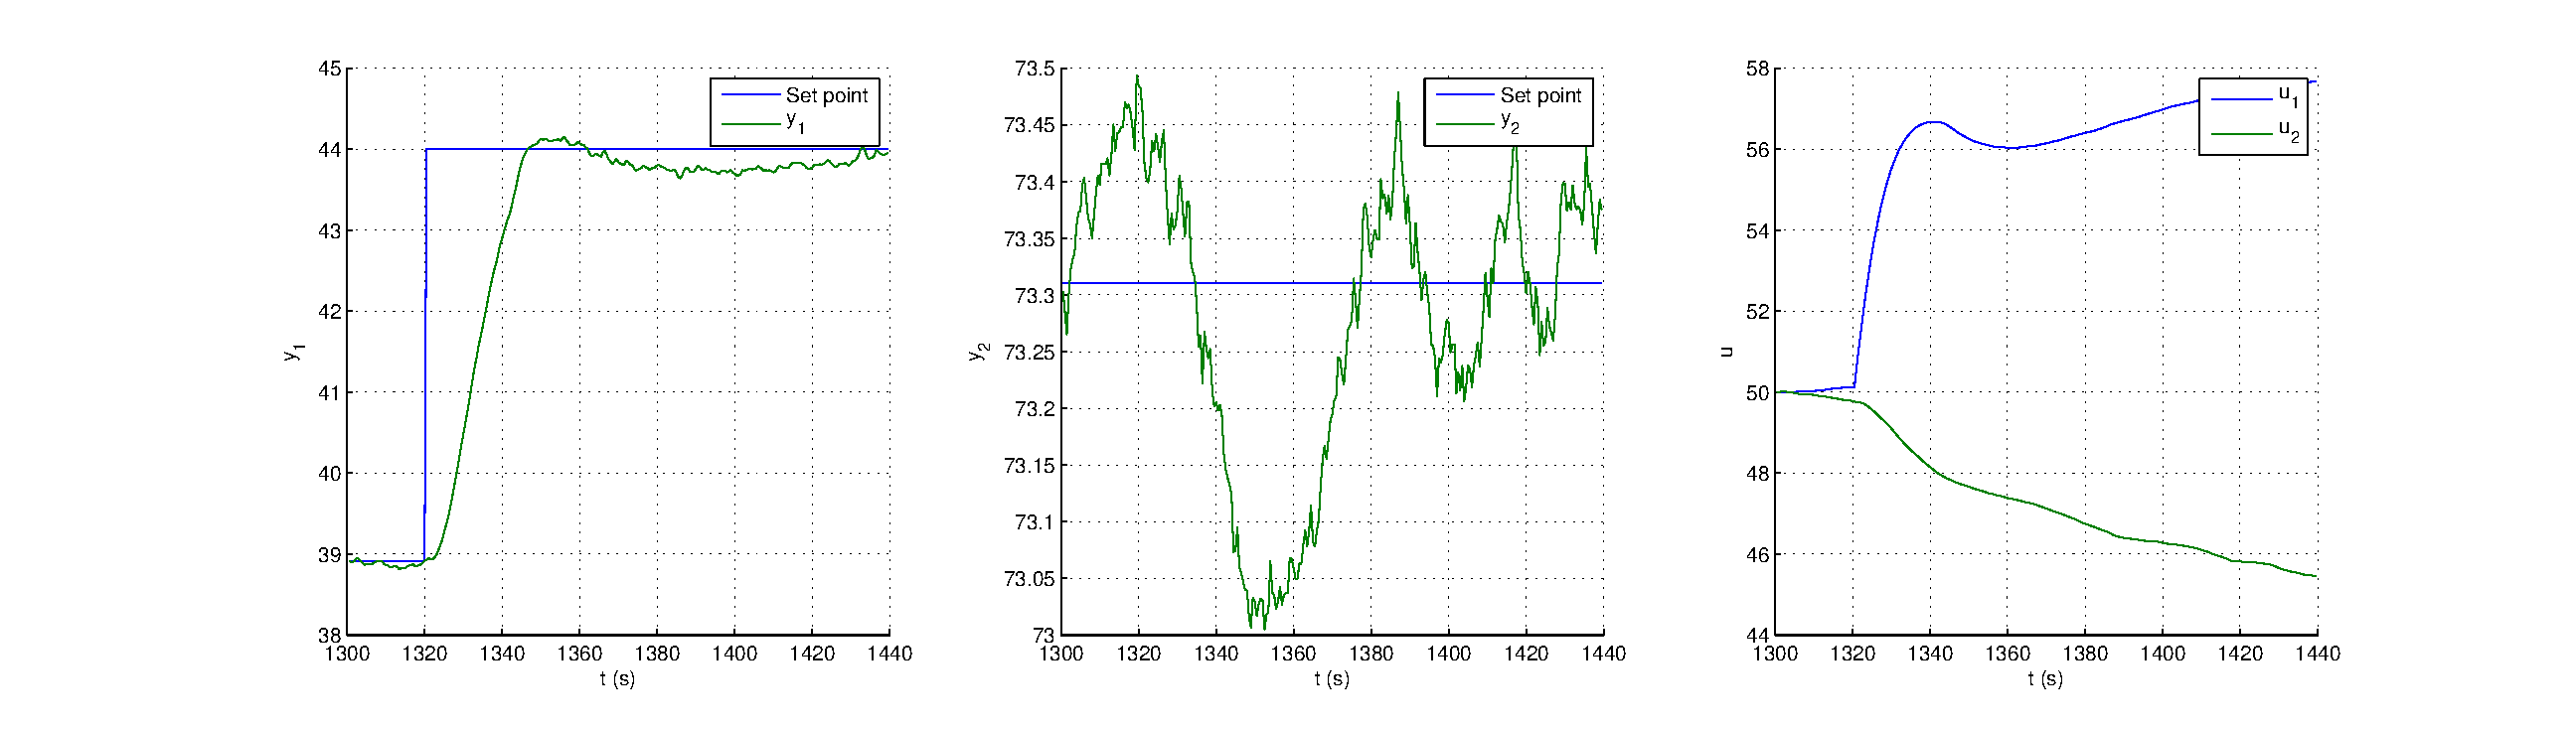
\includegraphics[width=\columnwidth]{fig/min_glover_step.eps}
                \caption{Step response}
        \end{subfigure}
        \begin{subfigure}[b]{\columnwidth}
                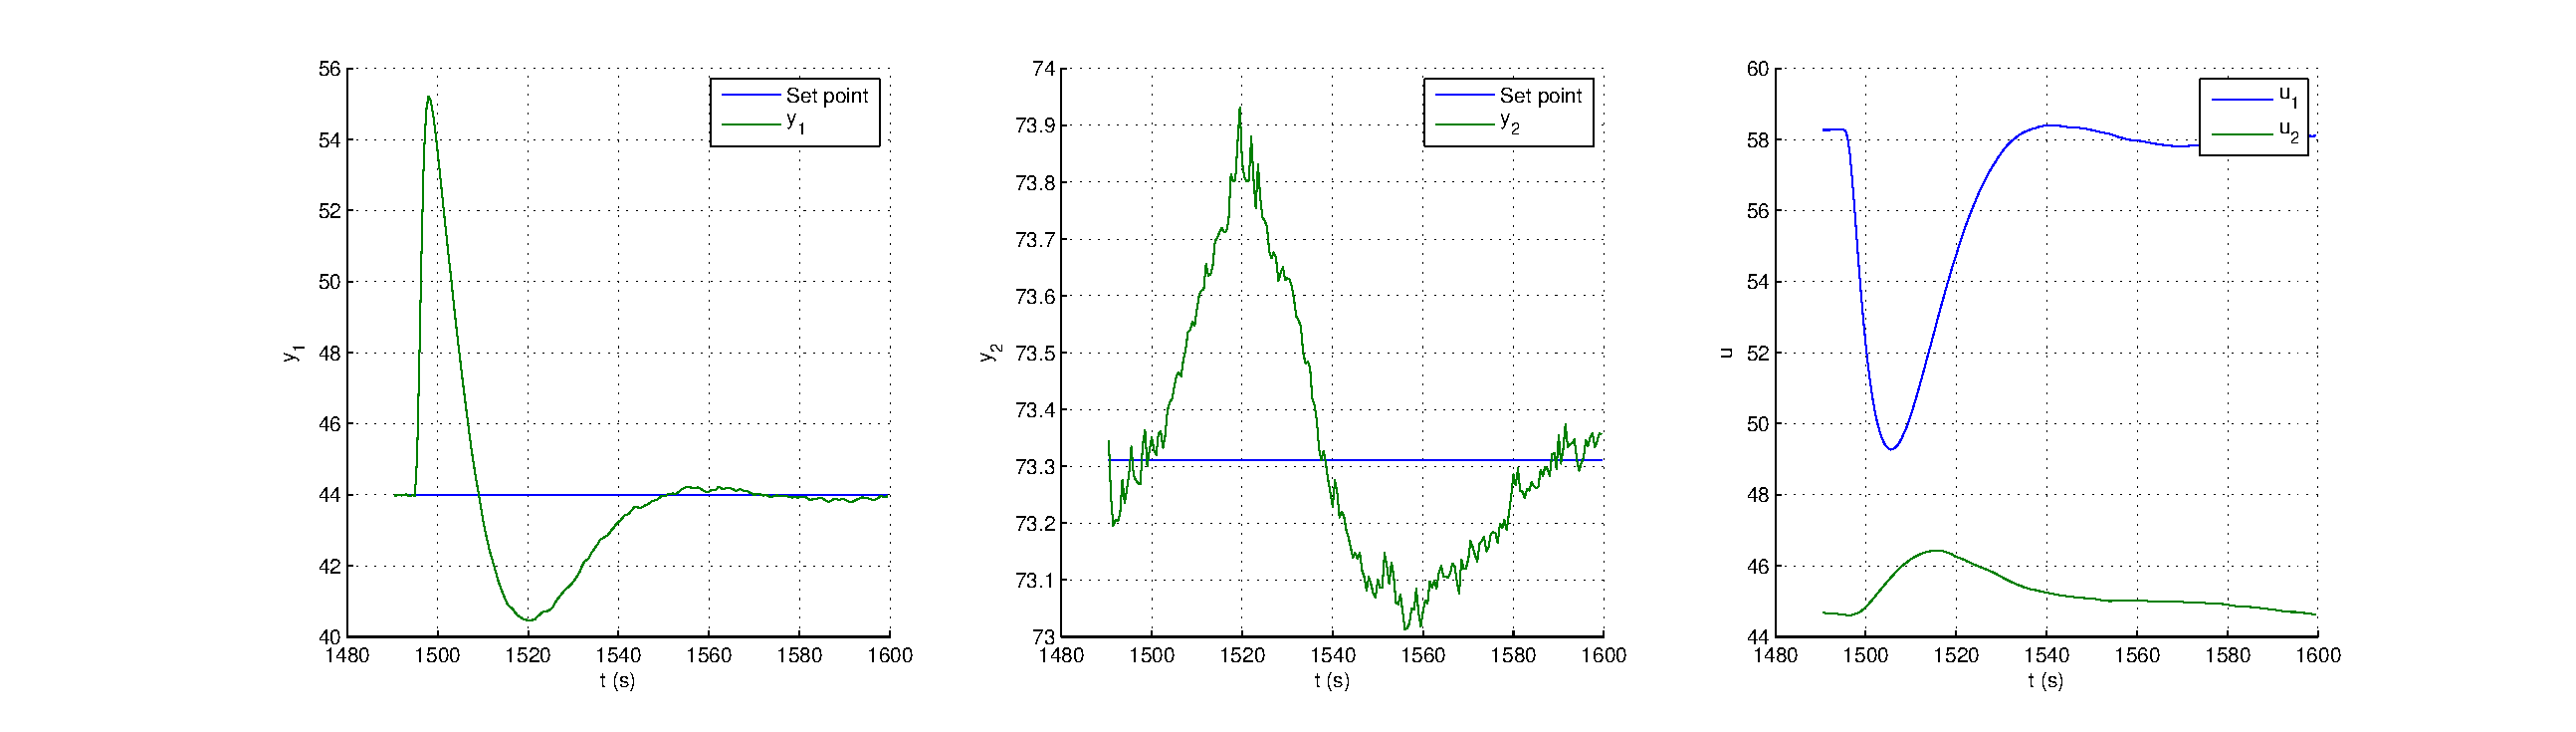
\includegraphics[width=\columnwidth]{fig/min_glover_gob.eps}
                \caption{Cup of water response}
        \end{subfigure}
        \begin{subfigure}[b]{\columnwidth}
                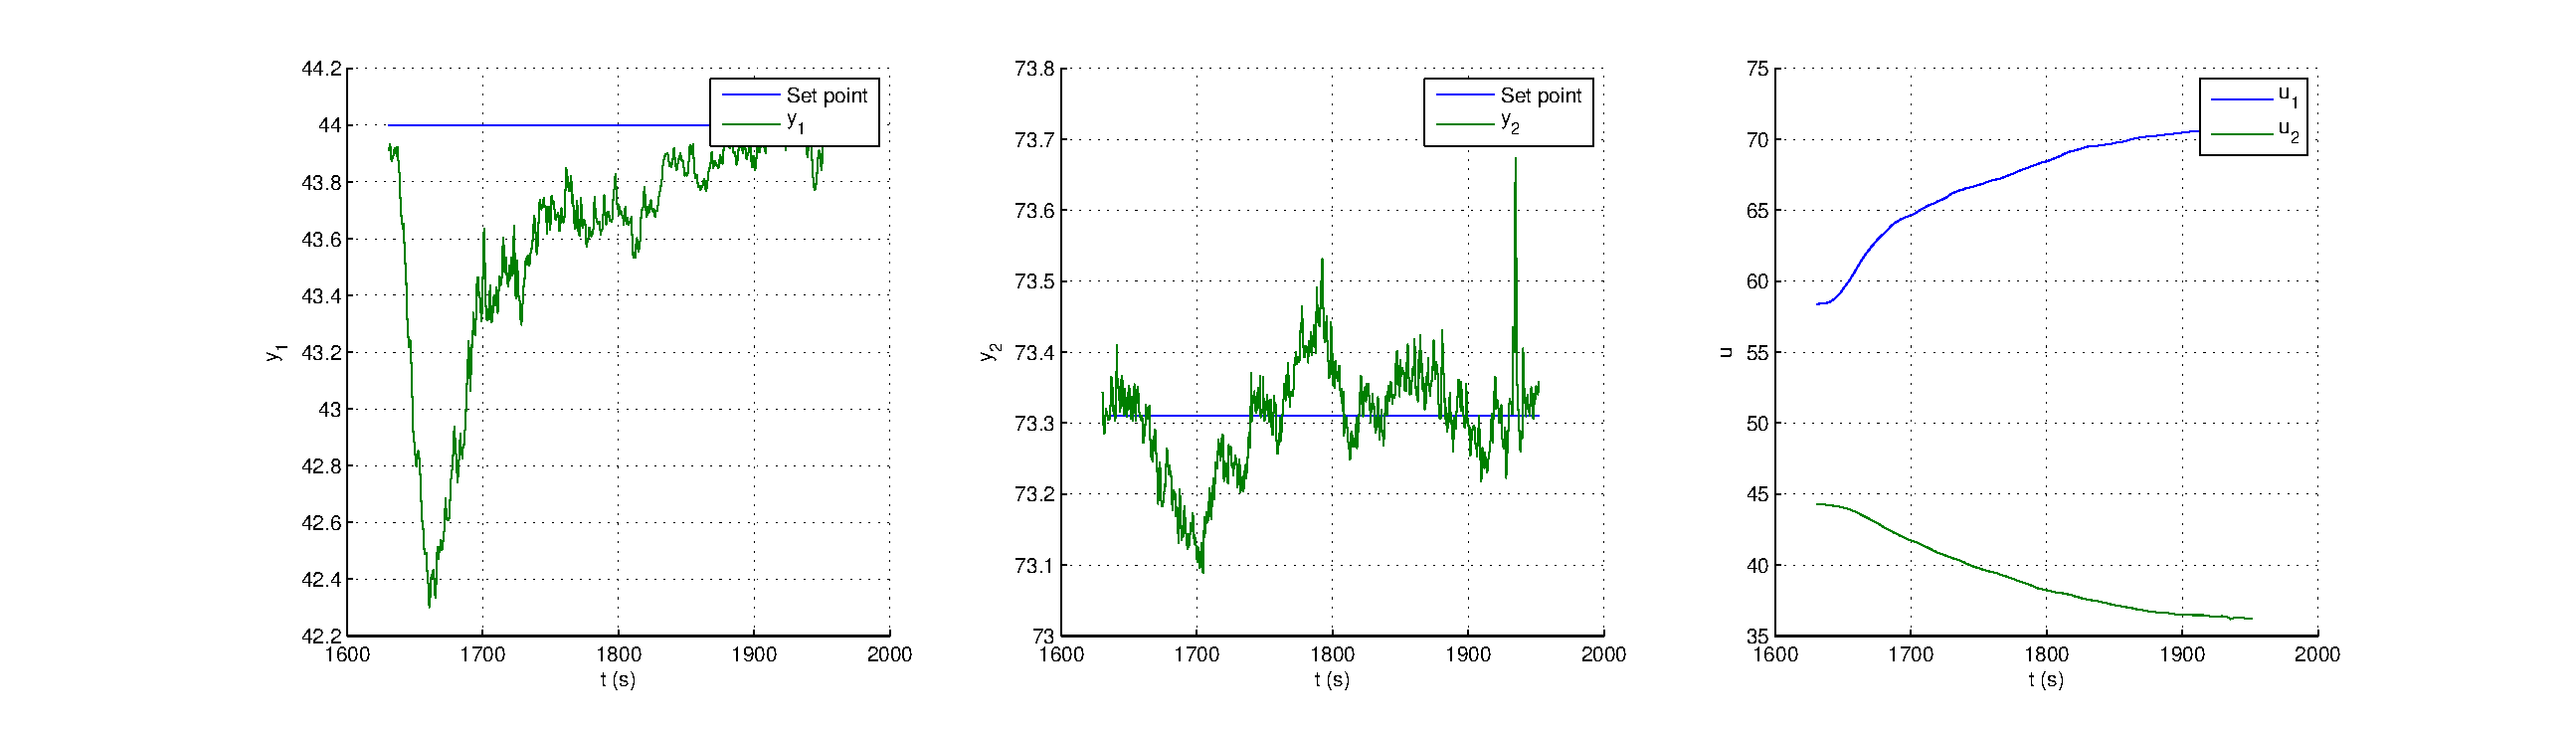
\includegraphics[width=\columnwidth]{fig/min_glover_fui.eps}
                \caption{Extra outlet response}
        \end{subfigure}
        \caption{Minimum phase system reactions \\ Glover-MacFarlane controller}
        \label{min_glover_fig}
\end{figure}

\begin{figure}[h!t]
        \centering
        \begin{subfigure}[b]{\columnwidth}
                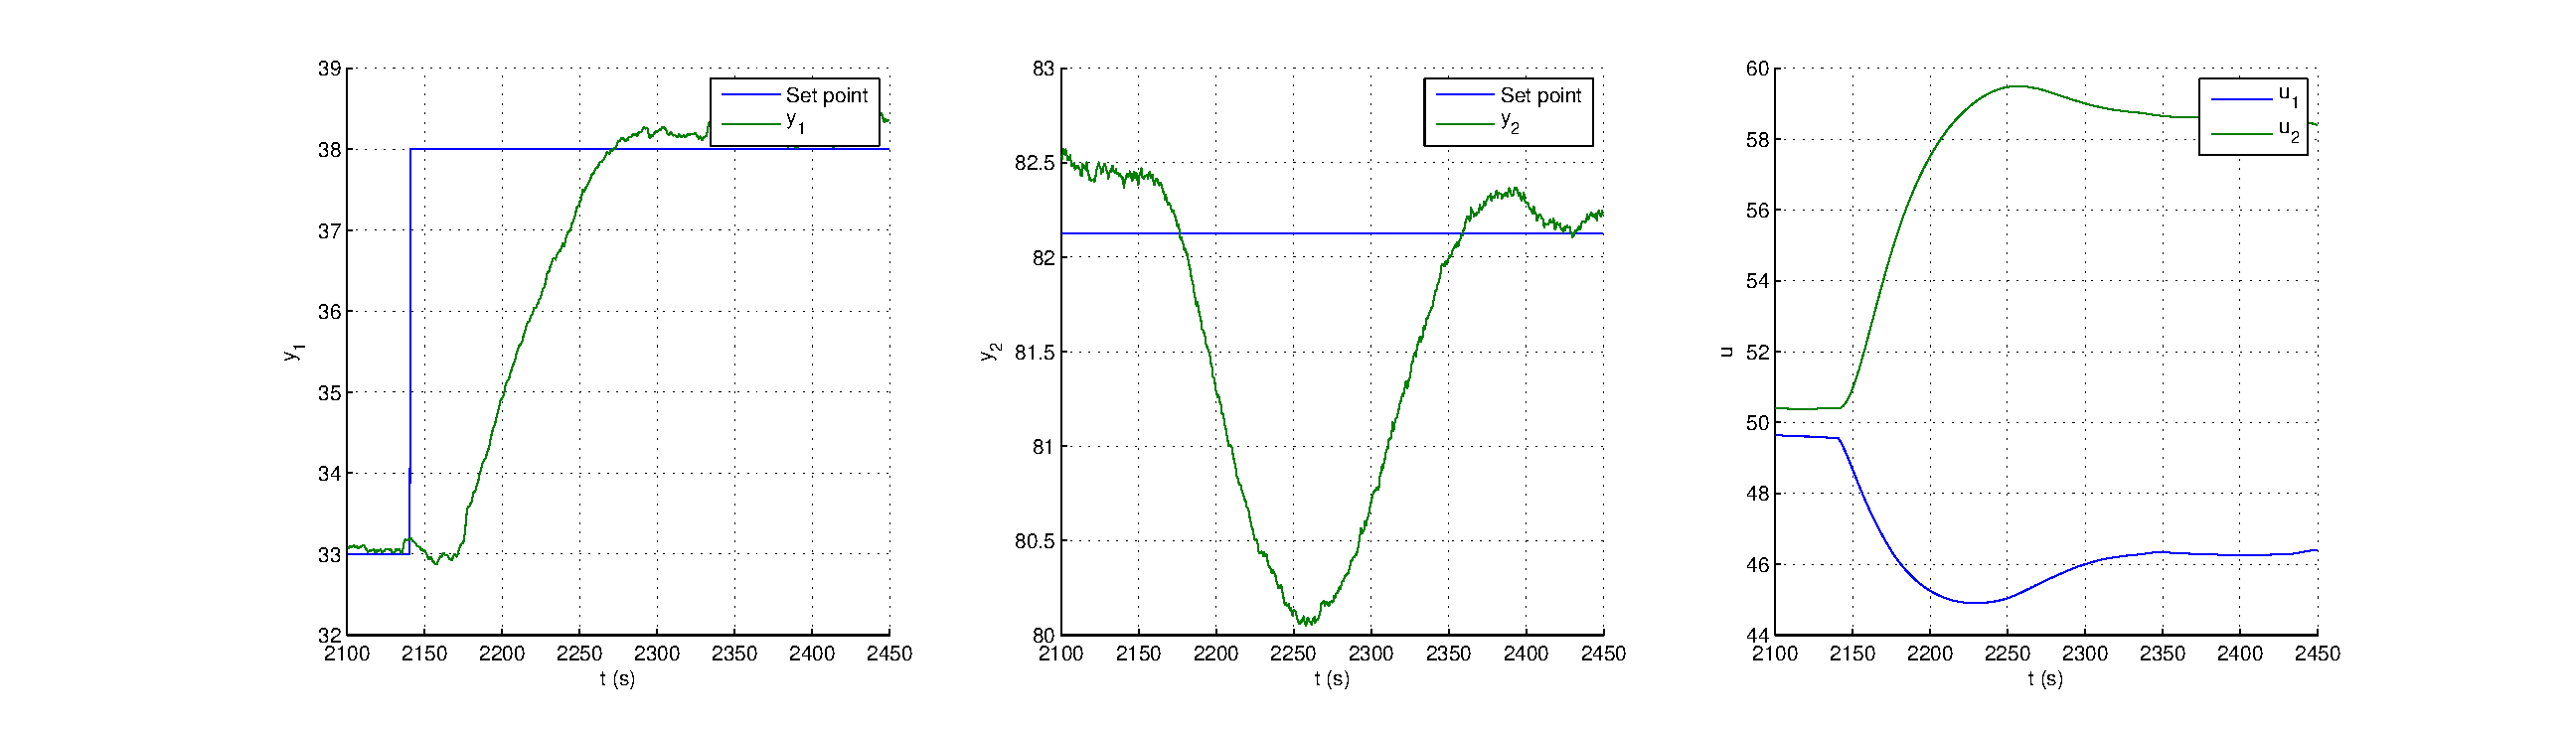
\includegraphics[width=\columnwidth]{fig/nonmin_glover_step.eps}
                \caption{Step response}
        \end{subfigure}
        \begin{subfigure}[b]{\columnwidth}
                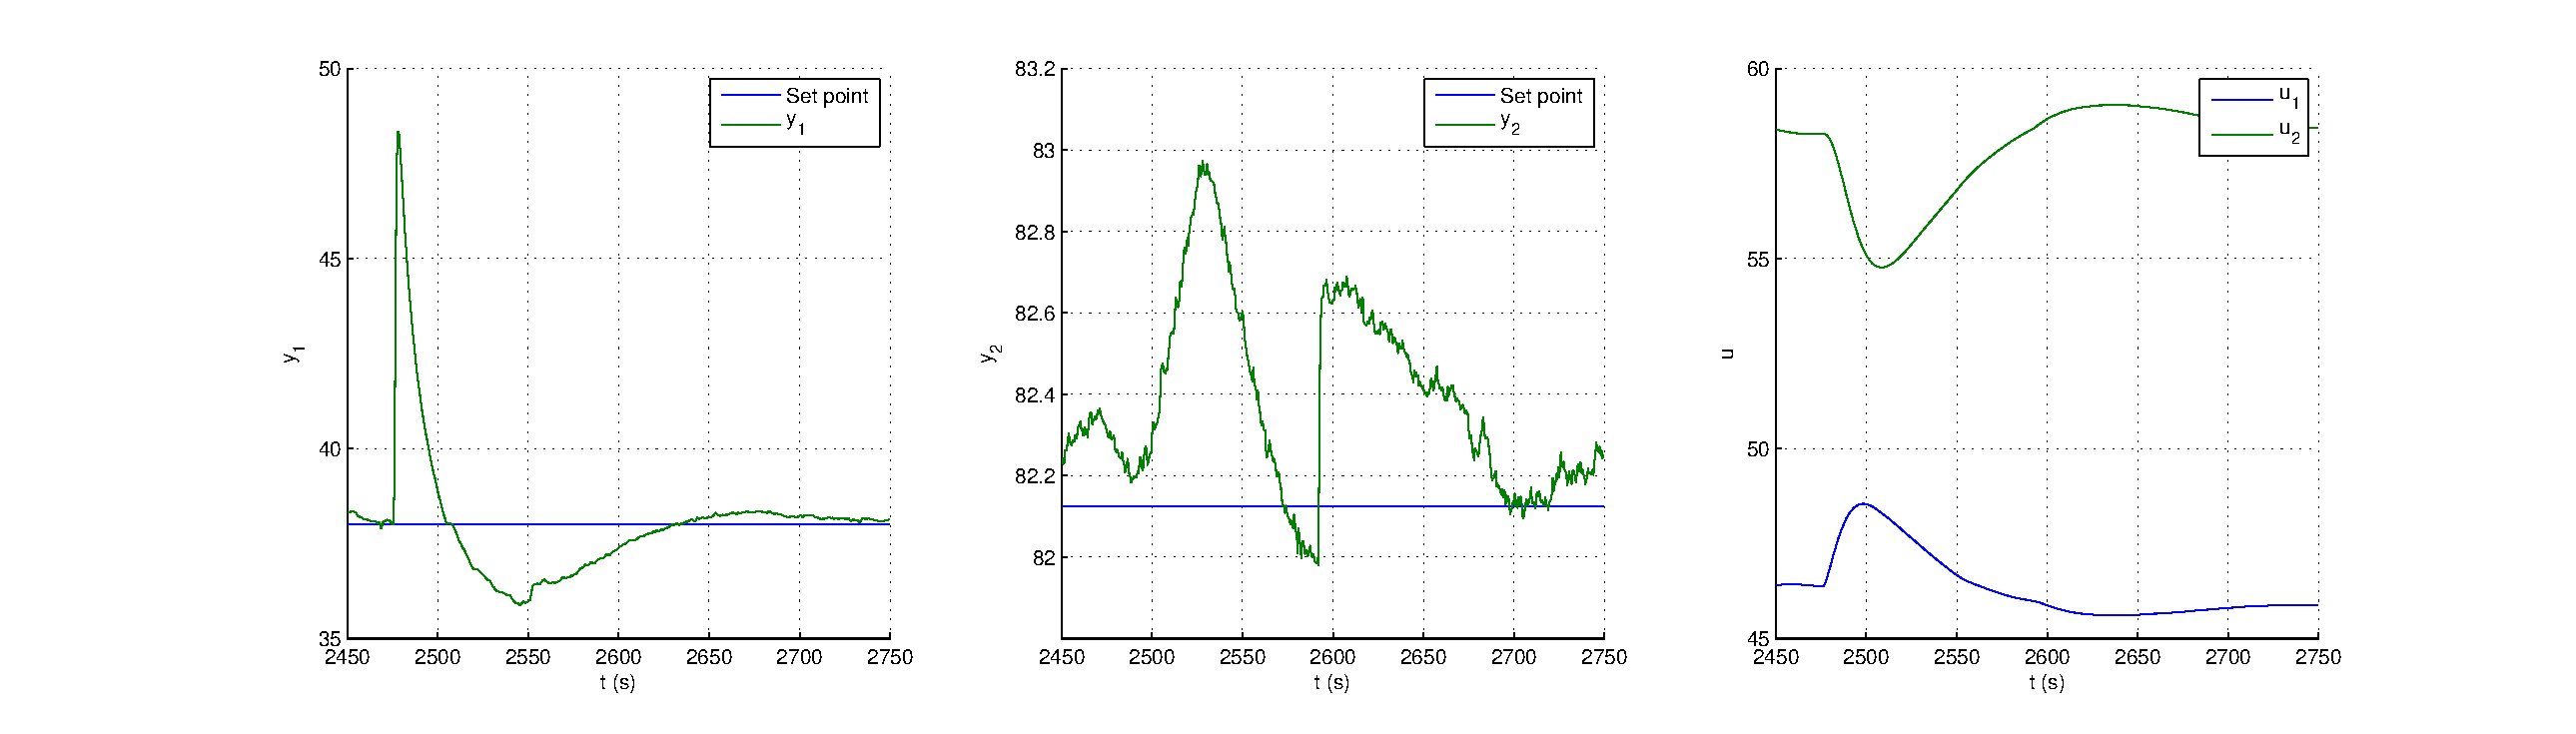
\includegraphics[width=\columnwidth]{fig/nonmin_glover_gob.eps}
                \caption{Cup of water response}
        \end{subfigure}
        \begin{subfigure}[b]{\columnwidth}
                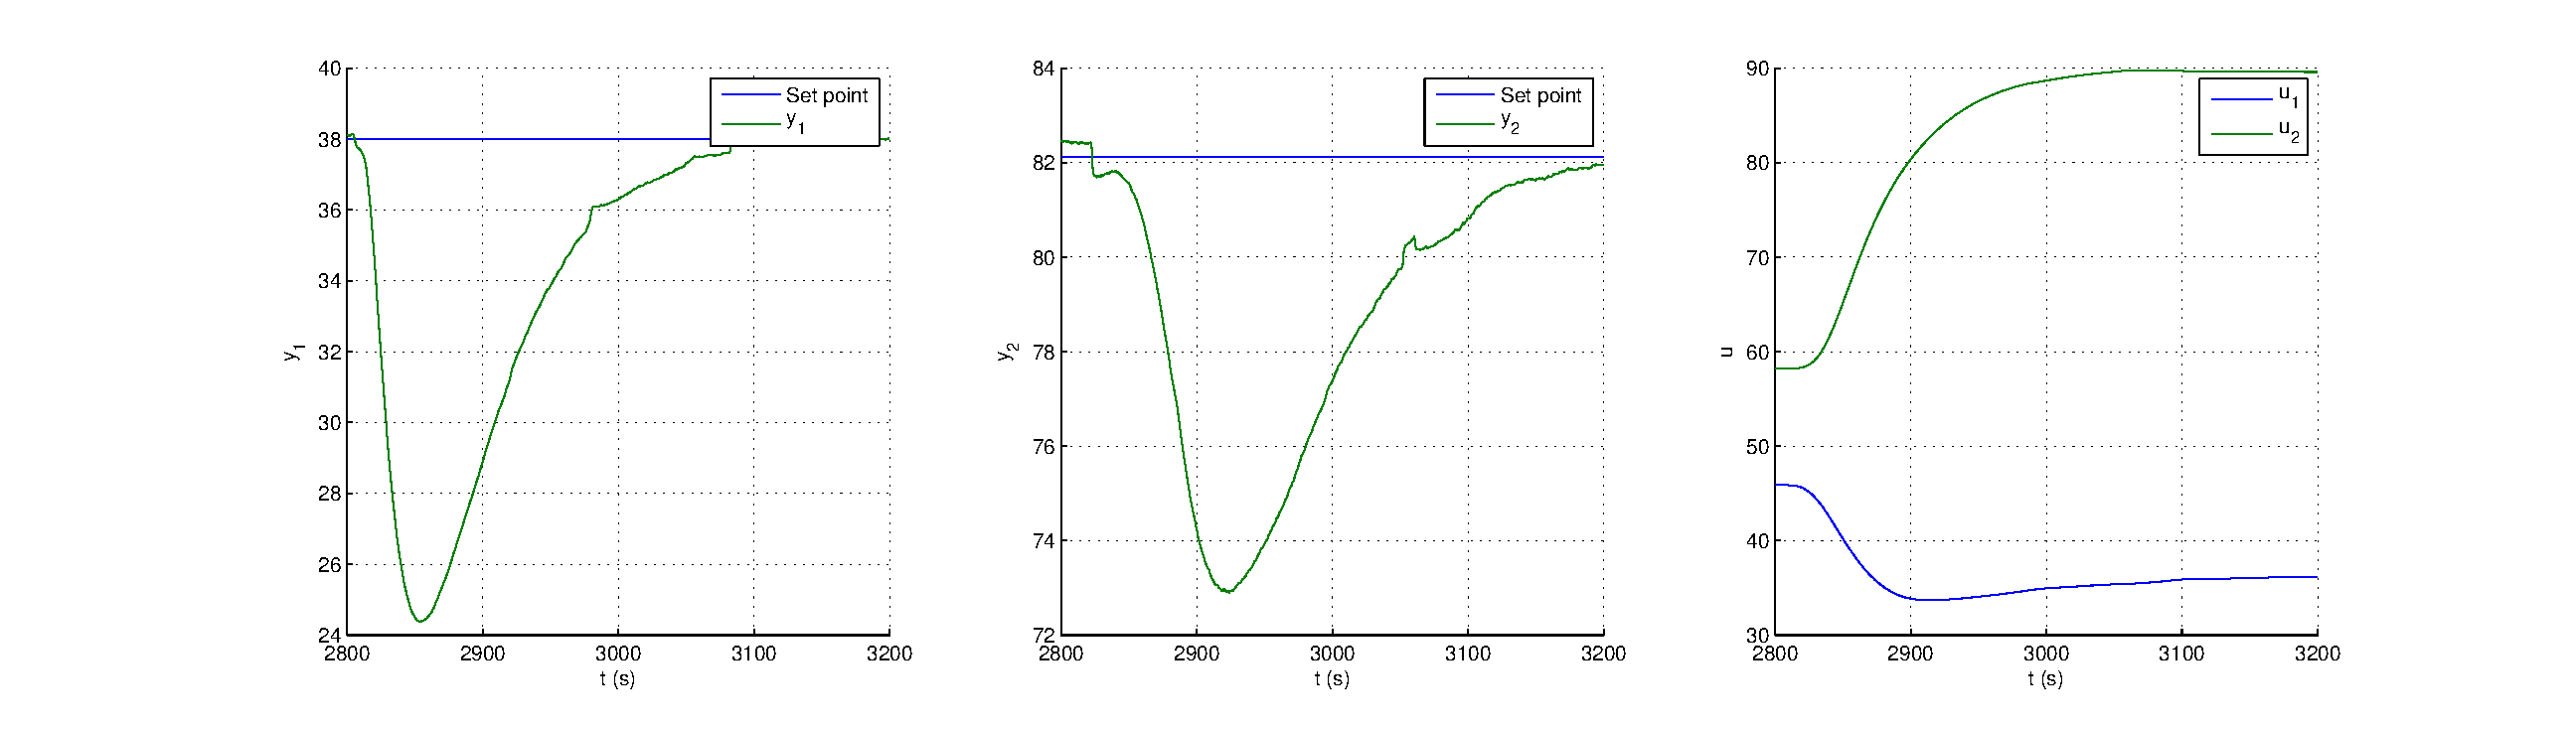
\includegraphics[width=\columnwidth]{fig/nonmin_glover_fui.eps}
                \caption{Extra outlet response}
        \end{subfigure}
        \caption{Non-minimum phase system reactions \\ Glover-MacFarlane controller}
        \label{nonmin_glover_fig}
\end{figure}

\begin{table}[h!t]
    \centering
    \begin{tabular}{|c|ccc|}
        \hline
        & Rise & \multirow{2}*{Overshoot} & Disturbance \\
        & time & & rejection \\
        Minimum phase & & & \\
        Non-minimum phase & & & \\
        \hline
    \end{tabular}
    \caption{Step response and load disturbance analysis \\ Glover-MacFarlane controllers}
    \label{analysis_glover}
\end{table}

\subsubsection{Exercise} 

Using Glover-MacFarlane controllers lead to a huge improvement of the controlled system:
\begin{shortitemize}
    \item All time are reduced (at least by a factor 2)
    \item Overshoots are decreased (at least by a factor 5)
    \item The step responses (non-minimum case) do not go in the wrong direction
\end{shortitemize}

% \subsubsection{Exercise}\lipsum[1-1]

% \subsubsection{Exercise}

The two previous exercises lead to the design of the following controller:

$$F_r(s) = \frac{1}{1 + \tau s}$$
$$F_y(s) = K \frac{\tau_D s + 1}{\beta \tau_D s +1}\frac{s + \omega_I}{s} \frac{\omega_0^2}{(s+\omega_0)^2}G(s)^{-1} G_d(s)$$

With:

$$\begin{array}{rcl}
    \tau & = & 0.14 \text{ s}\\ 
    K &  = & 1.35\\
    \tau_D &  = & 0.078\text{ s}\\
    \beta &  = & 0.75\\
 \omega_I &  = & 5 \text{ rad.s}^{-1}\\
    \omega_0 &  = & 50 \text{ rad.s}^{-1}\\
\end{array}$$

\textbf{All the criteria are met:}

\begin{shortitemize}
    \item Rise time:
        $$t_r = 0.19\text{s}$$
    \item Overshoot:
        $$D(\%) =  2.9\%$$
    \item Step in the disturbance:
        $$|y(t)| \leq 1, \forall t \text{ and } |y(t)| \leq 0.1, \forall t \geq 0.4\text{ s}$$ 
    \item Control signal obeys:
        $$|u(t)| \leq \max_t |u(t)| = 0.98 \leq 1, \forall t$$
\end{shortitemize}

Figure \ref{designFr} shows the step response of the system, the response to a step in the disturbance and the bode diagram of the sensitivity and complementary sensitivity functions.

\begin{figure}[h!t]
    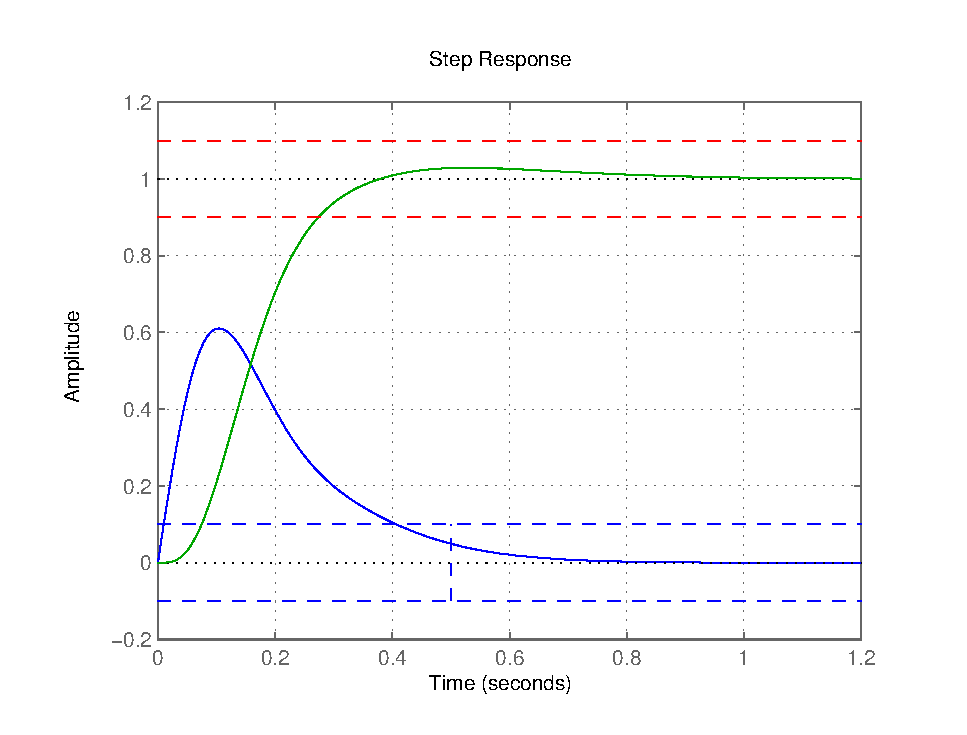
\includegraphics[width=\columnwidth]{fig/designFr.eps}
    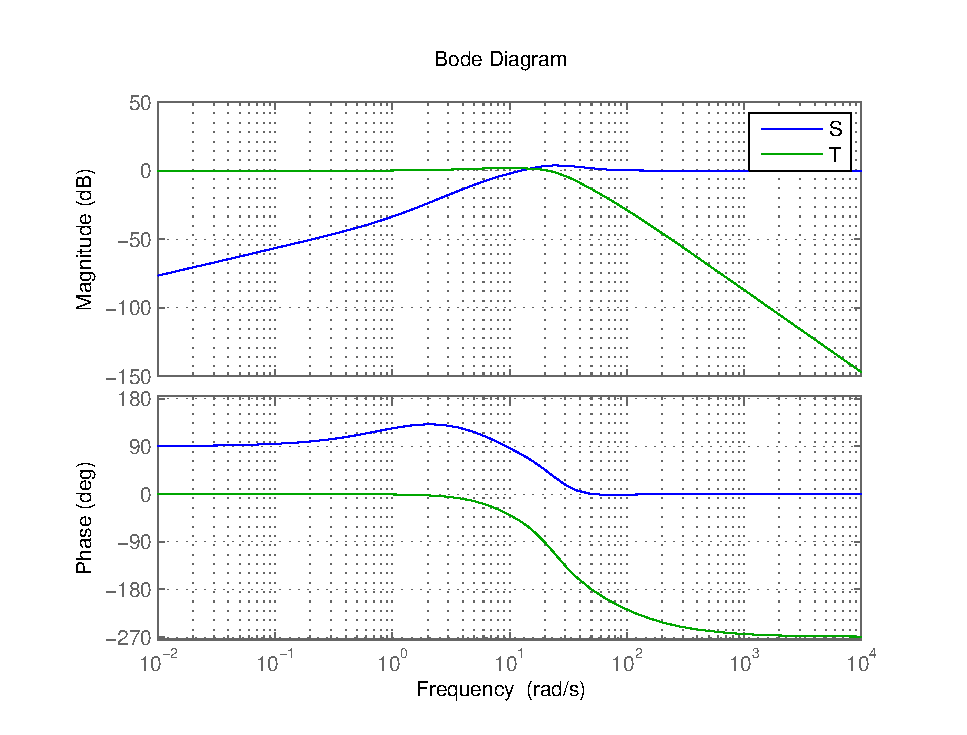
\includegraphics[width=\columnwidth]{fig/sensitivitiesFunction.eps}
    \caption{Step response of the system (green) and response to a step in the disturbance (blue) with the addition of the lead-controller \\ Bode diagram of the sensitivity and complementary sensitivity functions}
    \label{designFr}
\end{figure}


